\chapter{Numerical Simulations}
\label{chap:5}
Numerical Simulations are performed in order to have better understanding of system and for validation of control and steering law. For better system sizing a priory results from numerical simulations are important and very crucial in design process. Adaptive Runge Kutta method is used for numerical integration of nonlinear equation of motion. Customized software code is developed with ability to easily change system physical characteristics and constants in equation of motion. Developed code is capable to simulate Reaction Wheel, CMG individually and combination of both as VSCMG. Tests results are discussed for regulation and rest to rest with the vicinity of singular states.

\section{A priory dimensions}
Small form factor is considered utmost priority in design of test bench, hence starting with base platform considering which should fit under 250x250x250$\displaystyle mm^{3}$ and should not weigh more than 1.5kg. Apart from these test bed should also capable of carrying out maneuver with angular rate more than $\displaystyle 3^{\circ } /sec$. For preliminary understanding, parameters shown in \autoref{tbl:sys_param_pre} considered for simulations. 
\begin{table}[!h]
        \centering
        
\begin{tabular}{p{0.2\textwidth}|p{0.27\textwidth}|p{0.30\textwidth}|p{0.1\textwidth}}
\toprule
 Parameter & Symbol & Value & Unit \\
\midrule
 Skew Angle & $\displaystyle \beta $ & $\displaystyle 54.73$ & $\displaystyle deg$ \\

 Platform Inertia & $\displaystyle J_{P}$ & $\displaystyle diag([ 0.08,0.08,0.015])$ & $\displaystyle kg\cdotp m^{2}$ \\

 RW Inertia & $\displaystyle J^{s}_{W}$ & $\displaystyle 10\times 10^{-6}$ & $\displaystyle kg\cdotp m^{2}$ \\

 RW Inertia & $\displaystyle J^{g}_{W} ,\quad J^{t}_{W}$ & $\displaystyle 5\times 10^{-6}$ & $\displaystyle kg\cdotp m^{2}$ \\

 Gimbal Inertia & $\displaystyle J^{s}_{G} ,\ J^{t}_{G} ,\ J^{g}_{G}$ & $\displaystyle 3\times 10^{-6}$ & $\displaystyle kg\cdotp m^{2}$ \\

 CMG Inertia & $\displaystyle J^{s}_{CMG} ,\ J^{t}_{CMG} ,\ J^{g}_{CMG}$ & $\displaystyle diag([ 15,8,8]) \times 10^{-6}$ & $\displaystyle kg\cdotp m^{2}$ \\
\bottomrule
\end{tabular}
        \caption{Preliminary system configuration and dimensions}
        \label{tbl:sys_param_pre}
        \end{table}

\section{RW based ACS}
This section covers results in order to verify the dynamical model and sizing of reaction wheel. Two cases ha been studied, rest to rest reorientation to cancel attitude error and station keeping maneuver with initial angular velocity error.
\subsection{Rest to rest reorientation with RW only}
Consider a case where satellite has to be reoriented $\displaystyle 60\ \deg$ about its yaw axis in order to point solar panels towards sun, maneuver has to be done only using RWs and as per state defined in \autoref{tbl:states_rw_rr_y60}. This yaw error should be canceled within 20 seconds in order to satisfy minimum agility required.


\begin{table}[!h]
        \centering
        
\begin{tabular}{p{0.15\textwidth}|p{0.30\textwidth}|p{0.2\textwidth}}
\toprule
 Parameter & Value & Unit \\
\midrule
 $\displaystyle q$ & $\displaystyle [ 1\ 0\ 0\ 0]^{T}$ & - \\

 $\displaystyle \omega $ & $\displaystyle [ 0\ 0\ 0]^{T}$ & $\displaystyle \deg /\sec$ \\

 $\displaystyle q_{d}$ & $\displaystyle [\cos( \pi /6) \ 0\ 0\ \sin( \pi /6)]^{T}$ & - \\

 $\displaystyle \omega_d $ & $\displaystyle [ 0\ 0\ 0]^{T}$ & $\displaystyle rad/\sec$ \\

 $\displaystyle \delta $ & $\displaystyle [ 0\ 0\ 0\ 0]^{T}$ & $\displaystyle rad$ \\

 $\displaystyle \Omega $ & $\displaystyle [ 0\ 0\ 0\ 0]^{T}$ & $\displaystyle rad/\sec$ \\

 \bottomrule
\end{tabular}
        \caption{Initial and desired states with yaw error of $\displaystyle 60\deg$}
        \label{tbl:states_rw_rr_y60}
\end{table}

\begin{figure}[H]
     \centering
    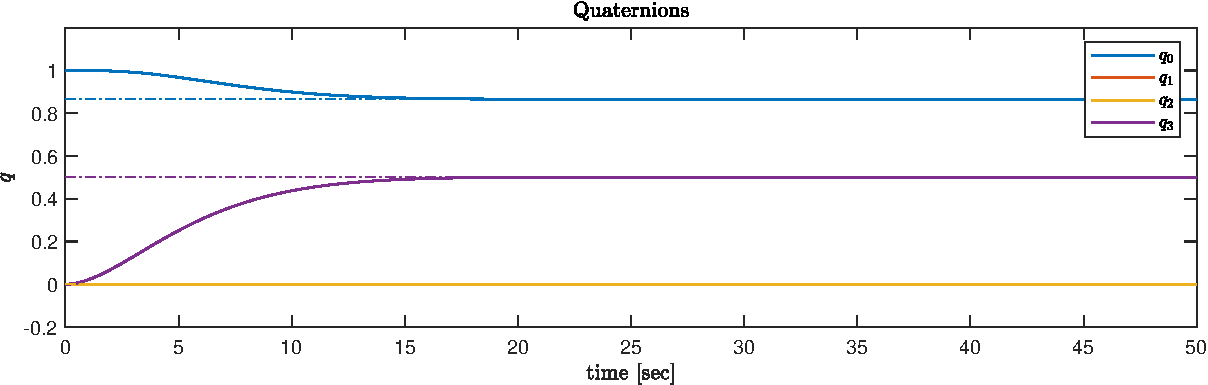
\includegraphics[width=1.0\columnwidth]{figures/plots/RW/rw_rr_y60_q.pdf}
    \caption{Quaternions for RW only rest to rest maneuver}
    \label{plt:rw_rr_y60_q_1}
\end{figure}
\noindent \autoref{plt:rw_rr_y60_q_1} to \autoref{plt:rw_rr_y60_Om_dot_1} are results
for given conditions in \autoref{tbl:states_rw_rr_y60}. It is clear from \autoref{plt:rw_rr_y60_q_1} that system approaches steady state within 20 seconds. Controller gains are selected such that attitude in terms of Euler angle is shown in \autoref{plt:rw_rr_y60_ypr_1} approaches reference yaw angle without overshoot.
\begin{figure}[H]
    \centering
    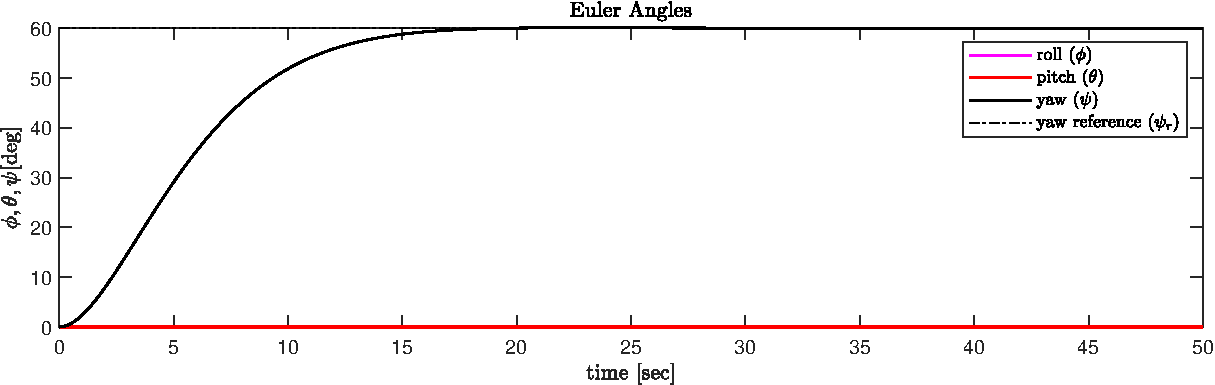
\includegraphics[width=0.9\columnwidth]{figures/plots/RW/rw_rr_y60_ypr.pdf}
    \caption{Euler angles for RW only rest to rest maneuver}
    \label{plt:rw_rr_y60_ypr_1}
\end{figure}

\begin{figure}[H]
    \centering
    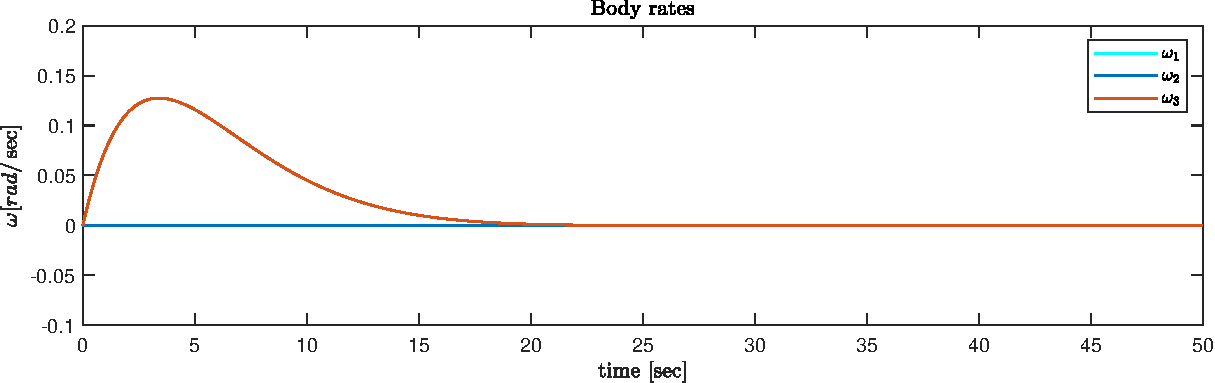
\includegraphics[width=0.9\columnwidth]{figures/plots/RW/rw_rr_y60_w.pdf}
    \caption{Body rates for RW only rest to rest maneuver}
    \label{plt:rw_rr_y60_w_1}
\end{figure}

\noindent Notice in \autoref{plt:rw_rr_y60_w_1} body angular velocity about yaw third axis considered as yaw starts from $0 rad/\sec$. Peak angular velocity $0.125 rad/\sec \approx 7.16^\circ/\sec$ occurs near 4 seconds and overall satisfying agility criteria of $3^\circ/\sec$ by reaching steady state close to $20 \sec$.

\begin{figure}[H]
    \centering
    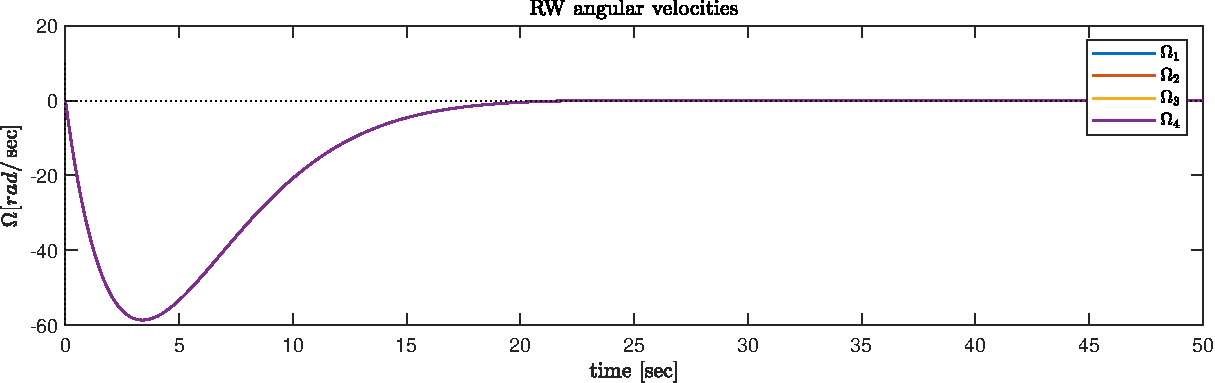
\includegraphics[width=0.9\columnwidth]{figures/plots/RW/rw_rr_y60_Om.pdf}
    \caption{RW velocity for RW only rest to rest maneuver}
    \label{plt:rw_rr_y60_Om_1}
\end{figure}

\begin{figure}[H]
    \centering
    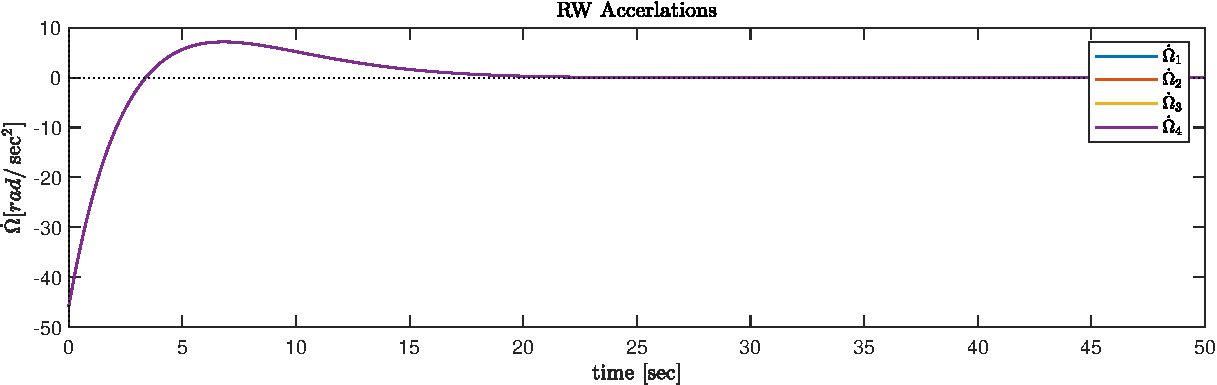
\includegraphics[width=0.8\columnwidth]{figures/plots/RW/rw_rr_y60_Om_dot.pdf}
    \caption{RW accelerations for RW only rest to rest maneuver}
    \label{plt:rw_rr_y60_Om_dot_1}
\end{figure}

\noindent All the reaction wheels rotated in same direction with almost equal rate which is understandable for given situation, maximum wheel speed is within reasonable range close to $60 rad/\sec \approx 570 RPM$, although initial RW acceleration starts from $-50 rad/\sec^2$ which probably should be smoothed by introducing proper gain scheduling, although these results are with preliminary assumption of geometrical properties and inertia and may change for final geometry.


\subsection{Regulation maneuver with RW only ACS}
Consider a scenario in which a satellite with configuration mentioned in \autoref{tbl:sys_param_pre} but subjected to small disturbance along body axis undergoes initial body rate error $\displaystyle \omega _{e} =[ -2\ 5\ 2]^{T} deg/sec$ \ has to counteract this error and should maintain its steady state such a way that asymptotic $\displaystyle q_{e} =[ 1\ 0\ 0\ 0]^{T}$. This is type of station attitude keeping maneuver often needs to performed when satellite deploy it's antenna or solar panel or subjected to impulse disturbance. Starting with same initial conditions from \autoref{tbl:states_rw_rr_y60} except $\displaystyle q_{d} =q=[ 1\ 0\ 0\ 0]^{T}$

\begin{figure}[H]
     \centering
    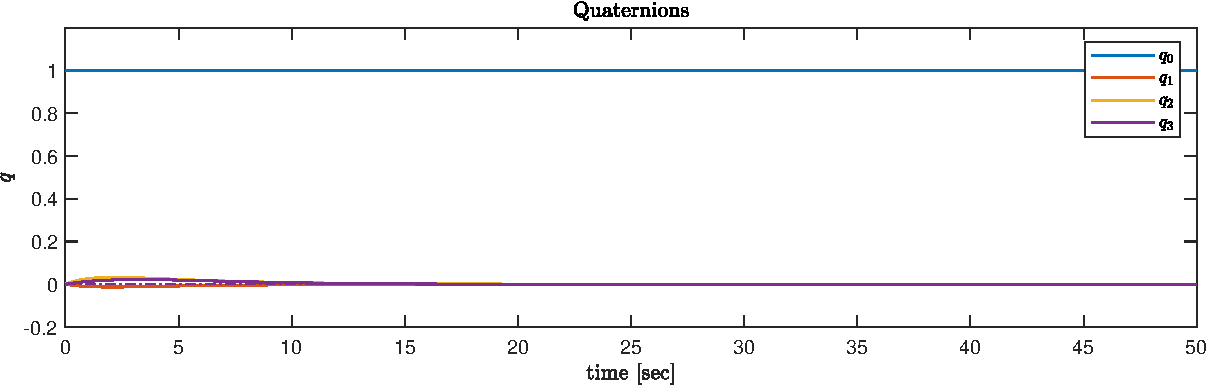
\includegraphics[width=0.8\columnwidth]{figures/plots/RW/rw_reg_w252_q.pdf}
    \caption{Quaternions for RW only station keeping maneuver}
    \label{plt:rw_reg_w252_q_1}
\end{figure}


\begin{figure}[H]
    \centering
    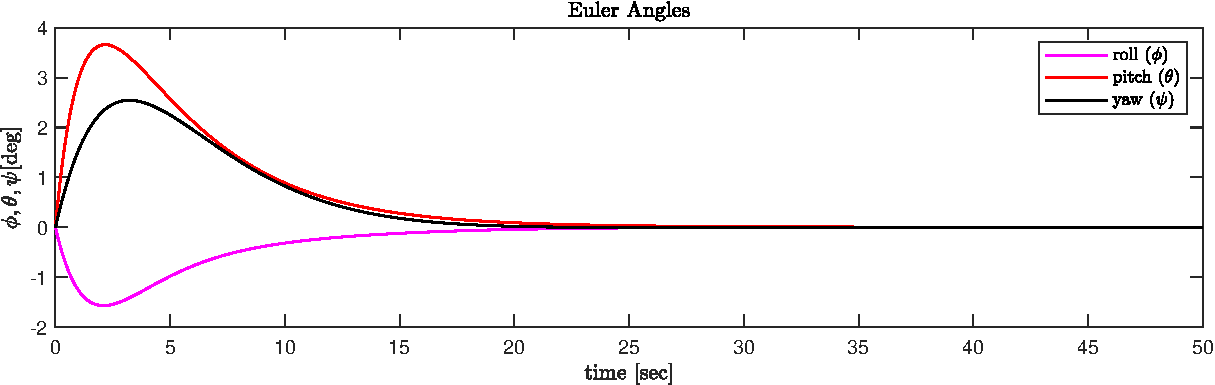
\includegraphics[width=0.8\columnwidth]{figures/plots/RW/rw_reg_w252_ypr.pdf}
    \caption{Euler angles for RW only station keeping maneuver}
    \label{plt:rw_rr_reg_w252_ypr_1}
\end{figure}
\noindent Results of initial body error problem are shown in \autoref{plt:rw_reg_w252_q_1} to  \autoref{plt:rw_rw_reg_w252_Om_dot_1}. We can note quaternion initially at rest are subjected to small variation and approaches its initial state in about 15 seconds. This is clearly visible in terms of Euler angles shown in \autoref{plt:rw_rr_reg_w252_ypr_1} all three angles roll pitch and yaw moved to peak angles approximately $ -1.5\degree, 3.5\degree $ and $ 2.4\degree $ respectively and slowly approaches to zero. Body rates shown in \autoref{plt:rw_reg_w252_w_1} starts from $ [-0.0349, 0.0873 0.0349] rad/sec$ smoothly approaches zero without showing any overshoot thanks to selected controller gain values. 

\begin{equation}
\mathbf{Kq} =\begin{pmatrix}
300 & 0 & 0\\
0 & 300 & 0\\
0 & 0 & 300
\end{pmatrix} ;\quad \mathbf{Kw} =\begin{pmatrix}
850 & 0 & 0\\
0 & 850 & 0\\
0 & 0 & 850
\end{pmatrix}
\label{eqn:RWO_gains}
\end{equation}

\noindent In \autoref{plt:rw_reg_w252_Om_1} notice how RW rates starting from zero diverge initially for 5 seconds and then maintain steady state velocities within range of -50 to 100 rad/sec although these are within the limit but may undergo saturation for large disturbances

\begin{figure}[H]
    \centering
    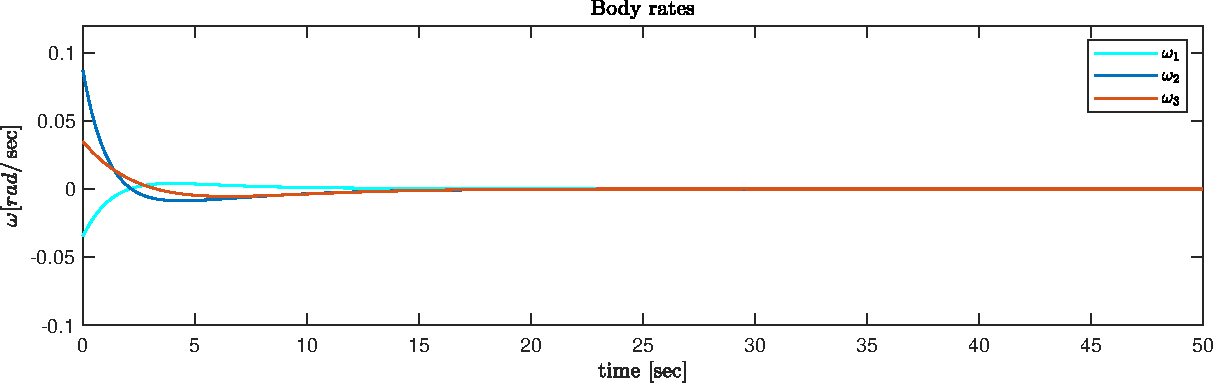
\includegraphics[width=0.9\columnwidth]{figures/plots/RW/rw_reg_w252_w.pdf}
    \caption{Body rates for RW only station keeping maneuver}
    \label{plt:rw_reg_w252_w_1}
\end{figure}


\begin{figure}[H]
    \centering
    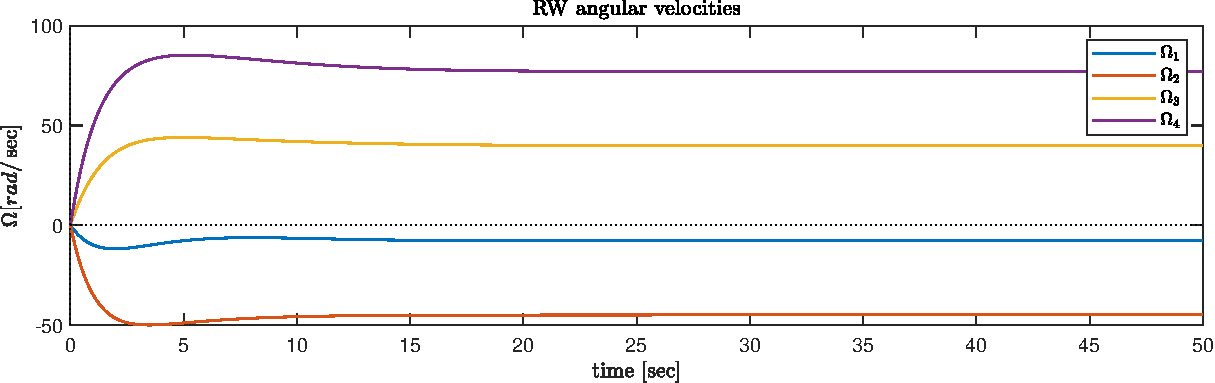
\includegraphics[width=0.9\columnwidth]{figures/plots/RW/rw_reg_w252_Om.pdf}
    \caption{RW velocity for RW only station keeping maneuver}
    \label{plt:rw_reg_w252_Om_1}
\end{figure}

\begin{figure}[H]
    \centering
    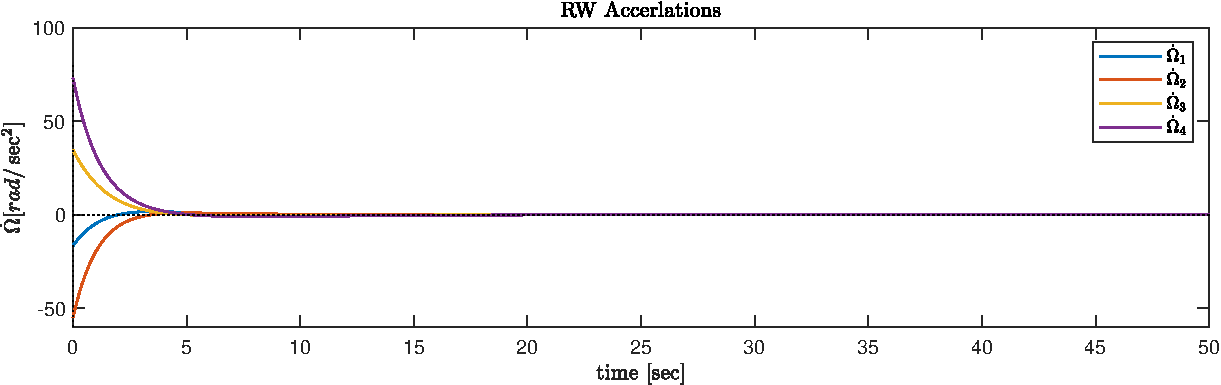
\includegraphics[width=0.9\columnwidth]{figures/plots/RW/rw_reg_w252_Om_dot.pdf}
    \caption{RW accelerations for RW only station keeping maneuver}
    \label{plt:rw_rw_reg_w252_Om_dot_1}
\end{figure}
\noindent From \autoref{plt:rw_rr_y60_Om_dot_1} we can see that Reaction wheels undergoes accelerations with magnitude up to $rad /\sec^2$ this parameter depends on inertia ratio of Platform to RW and can be reduced by either reducing platform inertia or by increasing RW inertia which is not suitable most of the time, thus torque amplification by CMG can be performed.
\section{CMG based ACS}
Despite the fact that RW based ACS is capable of eliminating attitude error in any direction, magnitude of torque produced is very low and limited by RW inertia, and may lead to saturation for large torque requirements. Subsequently, in the interest of taking advantage of torque amplification rest to rest and regulation maneuver are studied with CMG only control system.  
\subsection{Rest to rest reorientation with CMG only ACS}
Consider a satellite has to perform reorientation maneuver in order to cancel the attitude error in Euler angle $[\phi \ \theta \ \psi] = [30 \ 60 \ 90] \deg$ considering initial and desired states mentioned in \autoref{tbl:rr_ypr306090}


\begin{table}[!h]
        \centering
        
\begin{tabular}{p{0.15\textwidth}|p{0.40\textwidth}|p{0.15\textwidth}}
\toprule
 Parameter & Value & Unit \\
\midrule
 $\displaystyle q$ & $\displaystyle [ 1\ 0\ 0\ 0]^{T}$ & - \\
\hline 
 $\displaystyle \omega $ & $\displaystyle [ 0\ 0\ 0]^{T}$ & $\displaystyle \deg /\sec$ \\
\hline 
 $\displaystyle q_{d}$ & $\displaystyle [ 0.6830\ -0.1830\ 0.5000\ 0.5000]^{T}$ & - \\
\hline 
 $\displaystyle \omega _{d}$ & $\displaystyle [ 0\ 0\ 0]^{T}$ & $\displaystyle rad/\sec$ \\
\hline 
 $\displaystyle \delta $ & $\displaystyle \left[\frac{\pi }{2} ,\ \frac{\pi }{2} ,\ \frac{\pi }{2} ,\ \frac{\pi }{2}\right]^{T}$ & $\displaystyle rad$ \\
\hline 
 $\displaystyle \Omega $ & $\displaystyle [ 800,\ 800,\ 800,\ 800]^{T}$ & $\displaystyle rad/\sec$ \\
 \bottomrule
\end{tabular}
        \caption{Initial and desired states for attitude error $\displaystyle \phi =30\degree ,\theta =60\degree ,\ \psi =90\degree $}
\label{tbl:rr_ypr306090}
\end{table}
\noindent Time criterion for maneuver to be performed within 30 seconds will demonstrate performance beyond baseline agility requirement, and to do so Horowitz gains should be carefully selected for asymptotic stability. 


\begin{equation}
\mathbf{Kq} =\begin{pmatrix}
1 & 0 & 0\\
0 & 1 & 0\\
0 & 0 & 1
\end{pmatrix} ;\quad \mathbf{Kw} =\begin{pmatrix}
1.5 & 0 & 0\\
0 & 1.5 & 0\\
0 & 0 & 1.5
\end{pmatrix}
\label{eqn:CMO_gains}
\end{equation}
Notice gains selected for \acrshort{cmg} only \acrshort{acs} are much lower than those mentioned in \autoref{eqn:RWO_gains} selected for \acrshort{rw}  only \acrshort{acs}, we can infer that CMG can produce much higher torques compared with RW thus gain is reduced by order of magnitude of hundreds.

\begin{figure}[H]
     \centering
    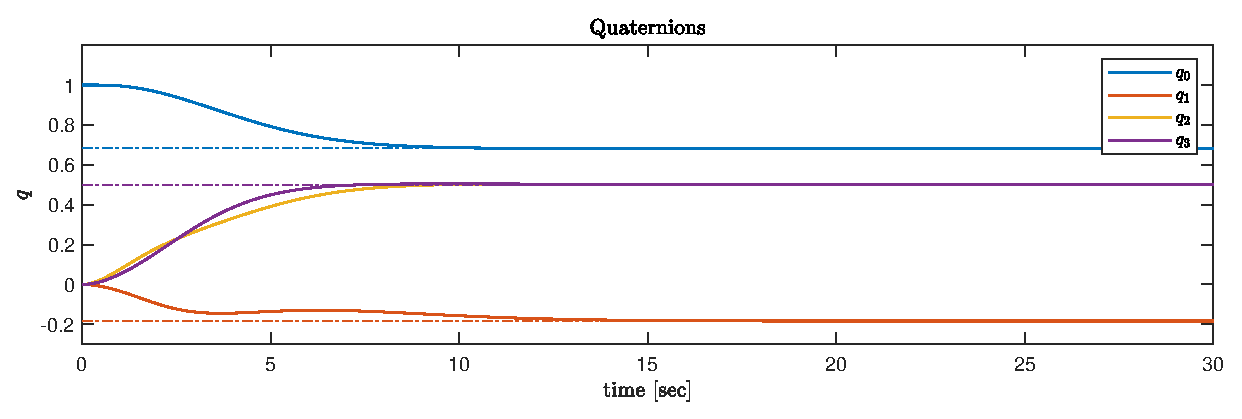
\includegraphics[width=0.9\columnwidth]{figures/plots/CMG/cm_rr_ypr369_q.eps}
    \caption{Quaternions for CMG only reorientation with attitude error $\displaystyle [\phi\ \theta\ \psi] =[30,\ 60,\ 90]\degree $}
    \label{plt:cm_rr_ypr369_q_2}
\end{figure}

\begin{figure}[H]
     \centering
    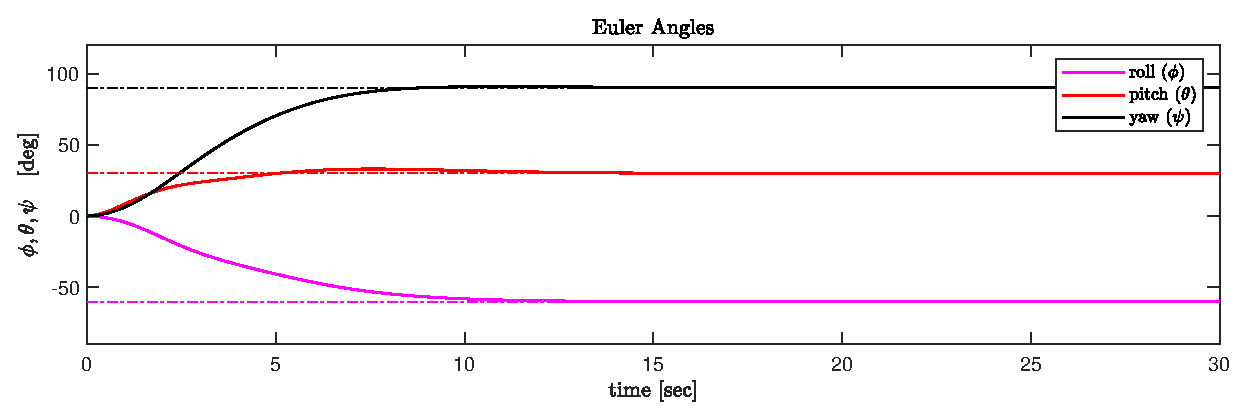
\includegraphics[width=0.9\columnwidth]{figures/plots/CMG/cm_rr_ypr369_ypr.eps}
    \caption{Euler angles for CMG only reorientation with attitude error $\displaystyle [\phi\ \theta\ \psi] =[30,\ 60,\ 90]\degree $}
    \label{plt:cm_rr_ypr369_ypr_2}
\end{figure}
\autoref{plt:cm_rr_ypr369_q_2} to \autoref{plt:cm_rr_ypr369_delta_dot_dot_2} are results for attitude error compensation maneuver with reference roll pitch yaw set as $\displaystyle [\phi\ \theta\ \psi] =[30,\ 60,\ 90]\degree $. Since gimbal state is far away from singularity, satellite smoothly approaches to reference states clearly seen from \autoref{plt:cm_rr_ypr369_q_2} and \autoref{plt:cm_rr_ypr369_ypr_2}.
\begin{figure}[H]
     \centering
    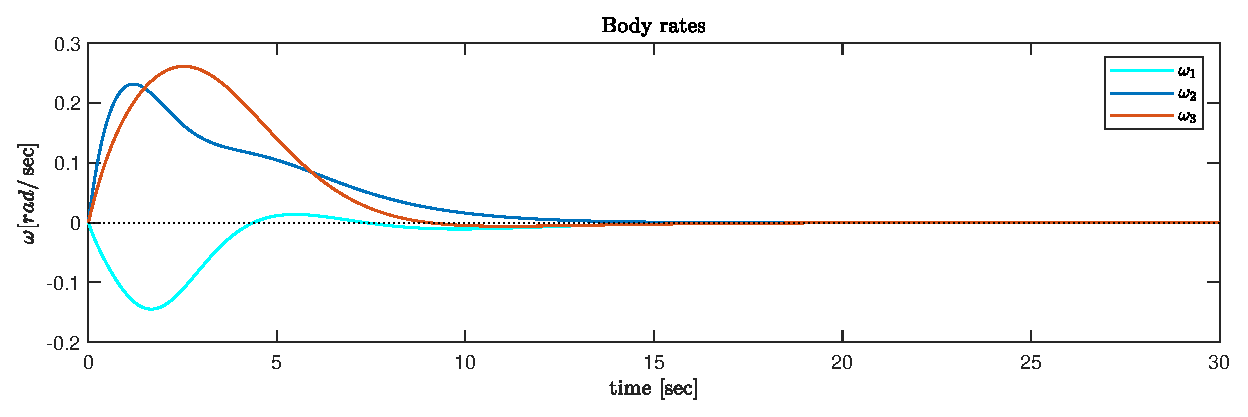
\includegraphics[width=0.9\columnwidth]{figures/plots/CMG/cm_rr_ypr369_w.eps}
    \caption{Body rates for CMG only reorientation with attitude error $\displaystyle [\phi\ \theta\ \psi] =[30,\ 60,\ 90]\degree $}
    \label{plt:cm_rr_ypr369_w_2}
\end{figure}
With negligible overshoot in body rate about third axis, satellite reaches steady state within 20 seconds seen in \autoref{plt:cm_rr_ypr369_w_2}. Gimbal angles initially set at $\pi/2 rad$ remains within magnitude of 1.2 to 1.9 radiance and no more than $20 \degree$ variation in gimbal angles is noticeable in \autoref{plt:cm_rr_ypr369_delta_2}. Although gimbal angular velocities shown in \autoref{plt:cm_rr_ypr369_delta_dot_2} has rapid variations which is understandable due to such a large slew motion is performed within 20 seconds.Moreover, smooth curves denotes CMG, was far away from singularity. 

\begin{figure}[H]
     \centering
    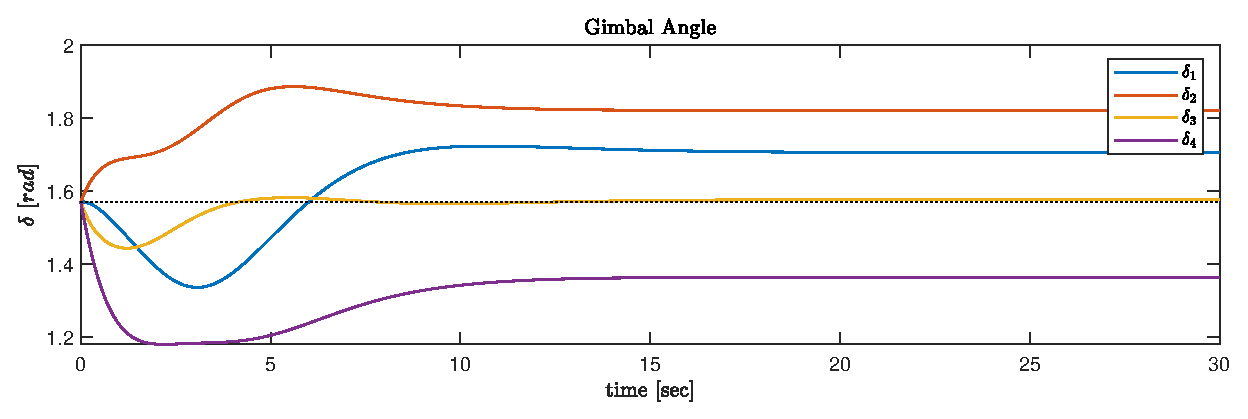
\includegraphics[width=0.9\columnwidth]{figures/plots/CMG/cm_rr_ypr369_delta.eps}
    \caption{Gimbal angles for CMG only reorientation with attitude error $\displaystyle [\phi\ \theta\ \psi] =[30,\ 60,\ 90]\degree $}
    \label{plt:cm_rr_ypr369_delta_2}
\end{figure}

\begin{figure}[H]
     \centering
    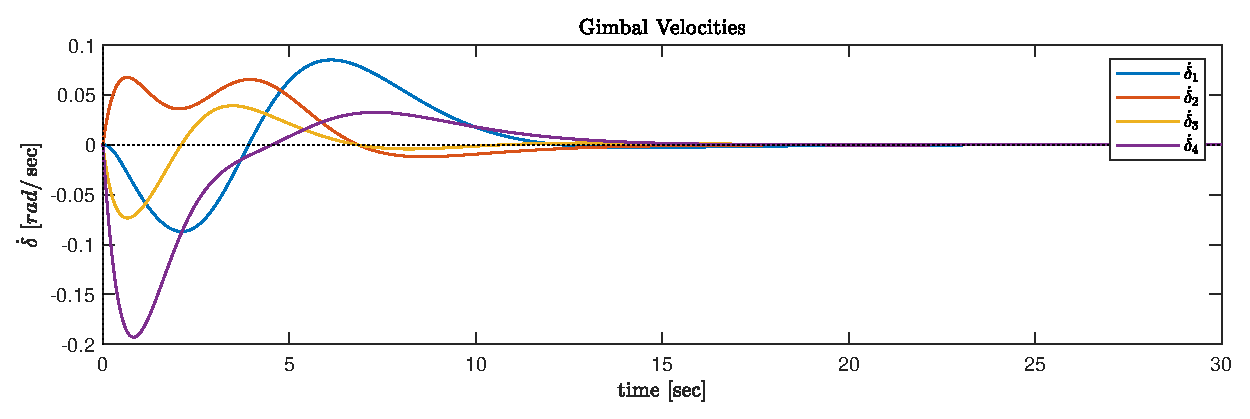
\includegraphics[width=0.9\columnwidth]{figures/plots/CMG/cm_rr_ypr369_delta_dot.eps}
    \caption{Gimbal rates for CMG only reorientation with attitude error $\displaystyle [\phi\ \theta\ \psi] =[30,\ 60,\ 90]\degree $}
    \label{plt:cm_rr_ypr369_delta_dot_2}
\end{figure}
\noindent Gimbal acceleration shown in \autoref{plt:cm_rr_ypr369_delta_dot_dot_2} are signals provided to gimbal motor in order to track required gimbal velocity for steering law. These accelerations are proportional to current supplied to gimbal motor. Acceleration magnitude is within range of $1 rad/\sec^2$ will not compromise the structural integrity of system.

\begin{figure}[H]
     \centering
    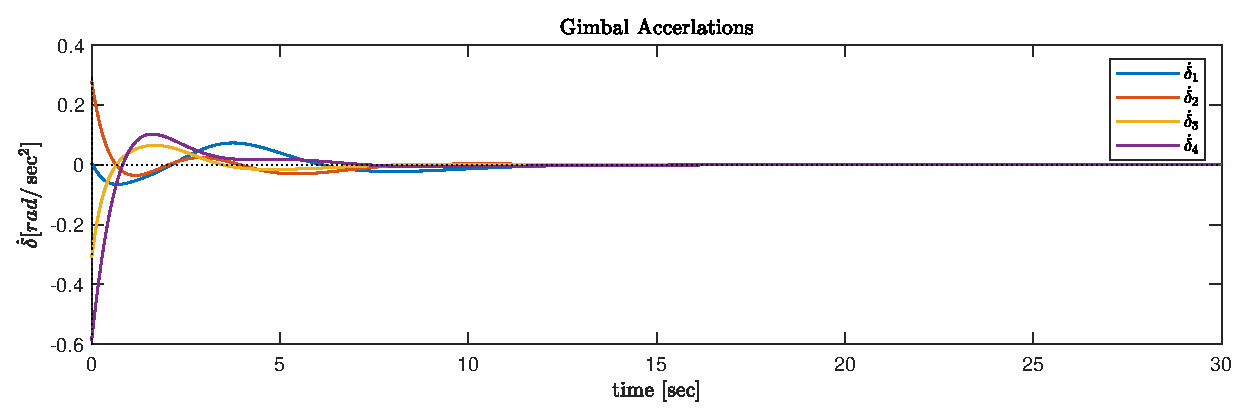
\includegraphics[width=0.9\columnwidth]{figures/plots/CMG/cm_rr_ypr369_delta_dot_dot.eps}
    \caption{Gimbal rates for CMG only reorientation with attitude error $\displaystyle [\phi\ \theta\ \psi] =[30,\ 60,\ 90]\degree $}
    \label{plt:cm_rr_ypr369_delta_dot_dot_2}
\end{figure}

\subsection{Body rate regulation with CMG only ACS}
Consider another scenario in which satellite is subjected to  step disturbance, ACS has to cancel angular velocity error and approach to its initial attitude, considering states from 


\begin{table}[!h]
        \centering
        
\begin{tabular}{p{0.15\textwidth}|p{0.40\textwidth}|p{0.15\textwidth}}
\toprule
 Parameter & Value & Unit \\
\midrule
 $\displaystyle q=q_{d}$ & $\displaystyle [ 1\ 0\ 0\ 0]^{T}$ & - \\
\hline 
 $\displaystyle \omega $ & $\displaystyle [ 0\ 10\ 0]^{T}$ & $\displaystyle \deg /\sec$ \\
\hline 
 $\displaystyle \omega _{d}$ & $\displaystyle [ 0\ 0\ 0]^{T}$ & $\displaystyle rad/\sec$ \\
\hline 
 $\displaystyle \delta $ & $\displaystyle [ 0,\ 0,\ 0,0]^{T}$ & $\displaystyle rad$ \\
\hline 
 $\displaystyle \Omega $ & $\displaystyle [ 800,\ 800,\ 800,\ 800]^{T}$ & $\displaystyle rad/\sec$ \\
 \bottomrule
\end{tabular}
\caption{Initial and desired states for angular velocity error with CMG in singular configuration}
\label{tbl_cmg_at_sing}
\end{table}
It is clear that CMG is at inescapable singularity thus combination of SVD bassed and off diagonal singularity avoidance steering law is used with gains selected by trial and error with numerous iterations.

\begin{equation}
\mathbf{Kq} =\begin{pmatrix}
5.3 & 0 & 0\\
0 & 5.3 & 0\\
0 & 0 & 5.3
\end{pmatrix} ;\quad \mathbf{Kw} =\begin{pmatrix}
2.5 & 0 & 0\\
0 & 2.5 & 0\\
0 & 0 & 2.5
\end{pmatrix}
\end{equation}
with using off diagonal singularity robust steering steering law as
\begin{equation}
\dot{\delta } =\mathbf{W}\mathcal{G}^{T}_{t}\left(\mathcal{G}_{t}\mathbf{W}\mathcal{G}^{T}_{t} +\lambda \mathbf{E}\right)^{-1} +\lambda \mathbf{v}_{1}
\end{equation}
where, weight matrices are selected by adding off diagonal harmonics as
\begin{equation*}
\mathbf{W} =\begin{pmatrix}
1 & \lambda  & \lambda  & \lambda \\
\lambda  & 2 & \lambda  & \lambda \\
\lambda  & \lambda  & 3 & \lambda \\
\lambda  & \lambda  & \lambda  & 4
\end{pmatrix}
\end{equation*}and
\begin{equation*}
\mathbf{E} =\begin{pmatrix}
100 & \epsilon _{3} & \epsilon _{2}\\
\epsilon _{3} & 100 & \epsilon _{1}\\
\epsilon _{2} & \epsilon _{1} & 100
\end{pmatrix}
\end{equation*}
with $ \epsilon _{i} =0.1\sin( \pi t+\varphi ) ,\ \varphi _{i} =\{0,\pi /2,\pi \}$ and $ \lambda =0.1\exp\left( -10\det\left(\mathcal{G}_{t}\mathcal{G}^{T}_{t}\right)\right)$ 
Results of CMG at singular states are shown in simulation \autoref{plt:cm_reg_w10_q} to \autoref{plt:zoom_plots_omega_sing}. Since CMG singularity is zero at the beginning satellite slowly diverges from set point, at first it performs complete $360 \degree$ rotation in yaw axis for about 245 seconds shown in \autoref{plt:cm_reg_w10_ypr}. Note that even there is discontinuity visible at 150 seconds, it is due to wrapping of Euler angles within range of -180$\degree$ to 180$\degree$ Rapid variation in body rate occurs, a spike seen near $250$ seconds in \autoref{plt:cm_reg_w10_w} and from zoomed view of body rate shown in \autoref{plt:cm_reg_w10_zoom_w} magnitude of about $1.5 rad/\sec$ occurs before reaching steady within next 10 seconds.
\begin{figure}[H]
     \centering
    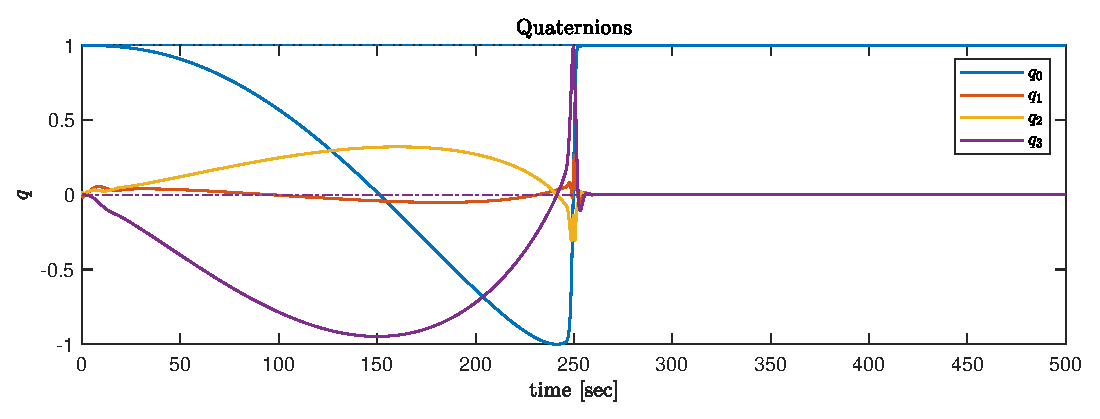
\includegraphics[width=0.9\columnwidth]{figures/plots/CMG/cm_reg_w10_q.eps}
    \caption{Quaternions for station keeping with CMG only ACS}
    \label{plt:cm_reg_w10_q}
\end{figure}

\begin{figure}[H]
     \centering
    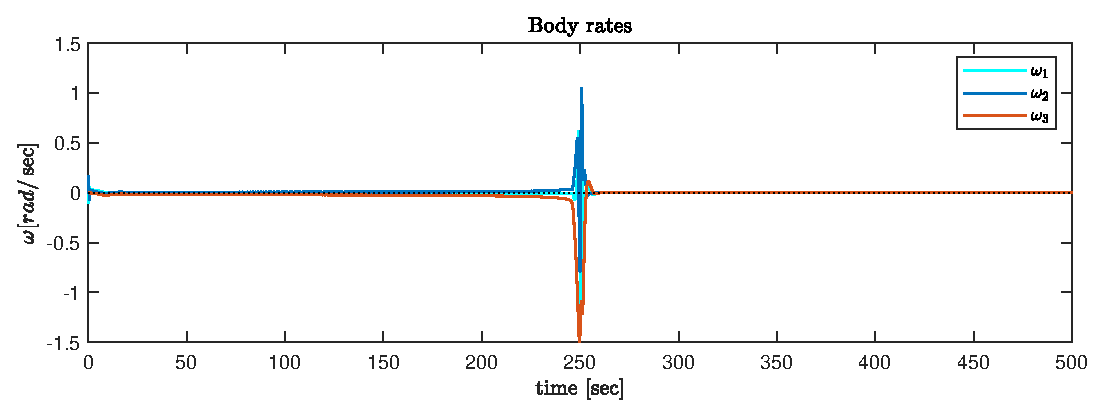
\includegraphics[width=0.9\columnwidth]{figures/plots/CMG/cm_reg_w10_w.eps}
    \caption{Body Rates for station keeping with CMG only ACS}
    \label{plt:cm_reg_w10_w}
\end{figure}



\begin{figure}[H]
     \centering
    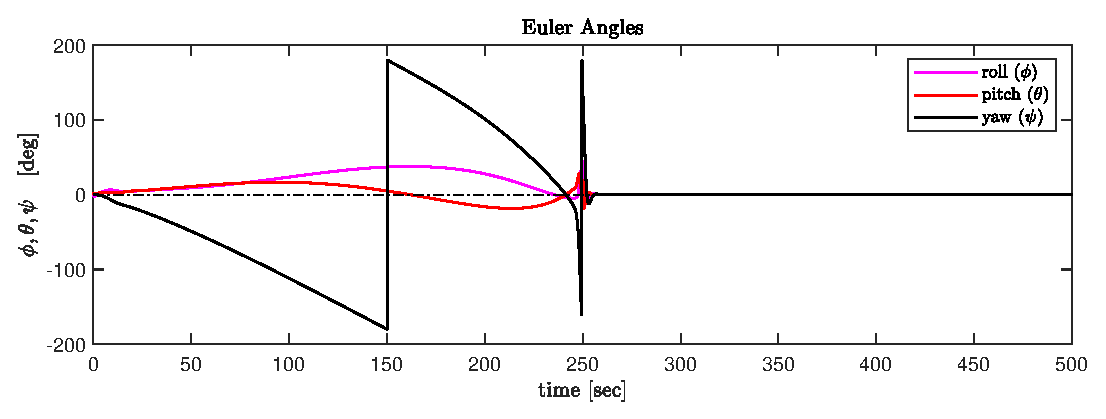
\includegraphics[width=0.9\columnwidth]{figures/plots/CMG/cm_reg_w10_ypr.eps}
    \caption{Euler angles for station keeping with CMG only ACS}
    \label{plt:cm_reg_w10_ypr}
\end{figure}
\noindent Gimbal angles slowly increase till 240 seconds and sudden jump occurs near 250 seconds. \autoref{plt:cm_reg_w10_delta_dot} and \autoref{plt:cm_reg_w10_zoom_delta_dot} are gimbal velocity and its zoomed view, notice how gimbal velocities rapidly change from 245 to 255 seconds Despite the fact that gimbal velocities are not exceptionally high, entire maneuver took about 270 seconds before reaching steady state which is not favorable. Thus being capable of producing large torque amplification, CMG alone can not guarantee smooth tracking performance. Moreover, finding perfect parameters and gains for particular task is not trivial since they vary depending on type of singularity and state.
\begin{figure}[H]
     \centering
    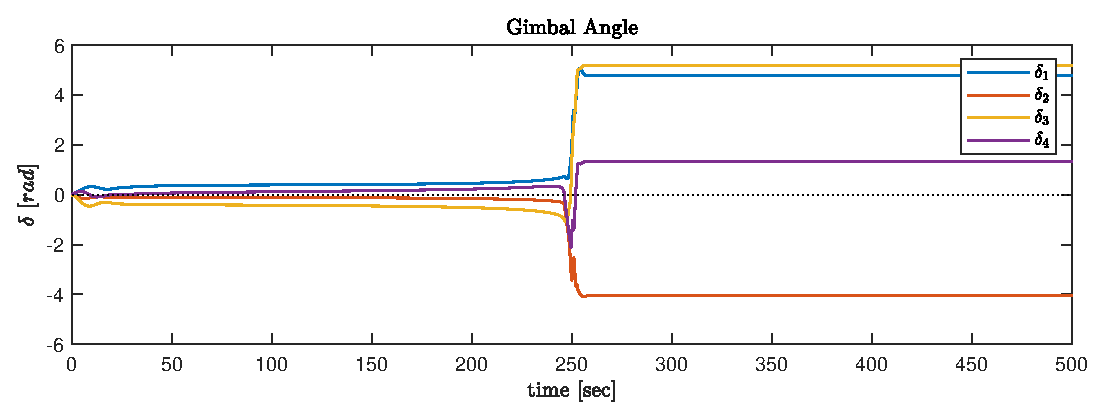
\includegraphics[width=0.9\columnwidth]{figures/plots/CMG/cm_reg_w10_delta.eps}
    \caption{Gimbal angles for station keeping with CMG only ACS}
    \label{plt:cm_reg_w10_delta}
\end{figure}

\begin{figure}[H]
     \centering
    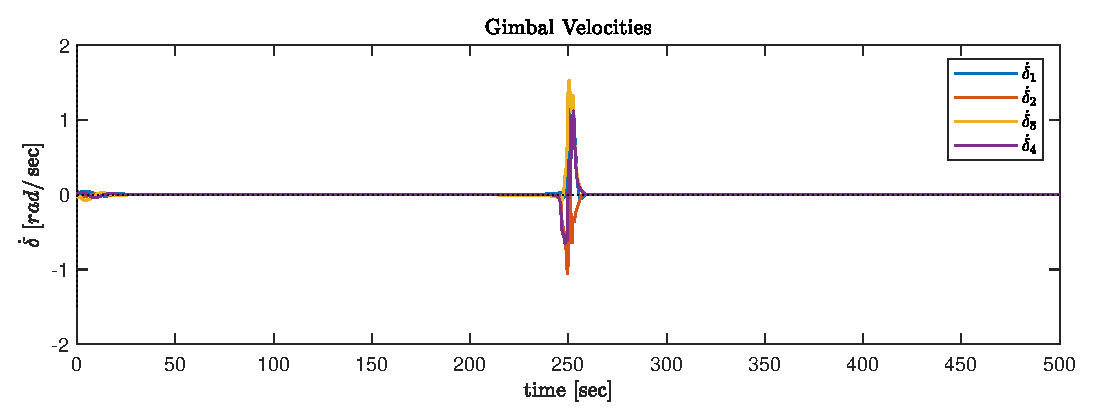
\includegraphics[width=0.9\columnwidth]{figures/plots/CMG/cm_reg_w10_delta_dot.eps}
    \caption{Gimbal velocities for station keeping with CMG only ACS}
    \label{plt:cm_reg_w10_delta_dot}
\end{figure}

\begin{figure}[H]
    \centering
  \begin{subfigure}[b]{0.49\columnwidth}
     \centering
    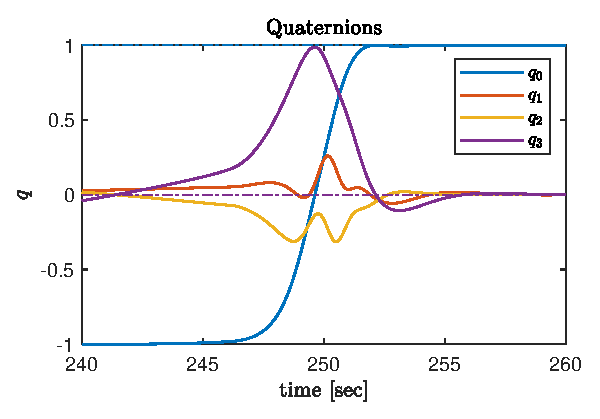
\includegraphics[width=1\columnwidth]{figures/plots/CMG/cm_reg_w10_zoom_q.eps}
    \caption{Quaternions}
    \label{plt:cm_reg_w10_zoom_q}
\end{subfigure}
  %
  \begin{subfigure}[b]{0.49\columnwidth}
     \centering
    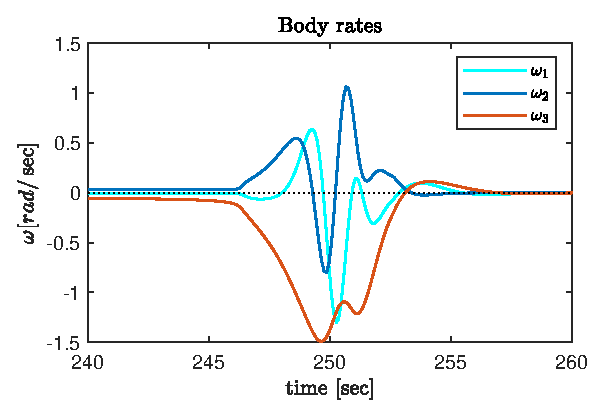
\includegraphics[width=1\columnwidth]{figures/plots/CMG/cm_reg_w10_zoom_w.eps}
    \caption{Body Rates}
    \label{plt:cm_reg_w10_zoom_w}
\end{subfigure}
  %
  \begin{subfigure}[b]{0.49\columnwidth}
     \centering
    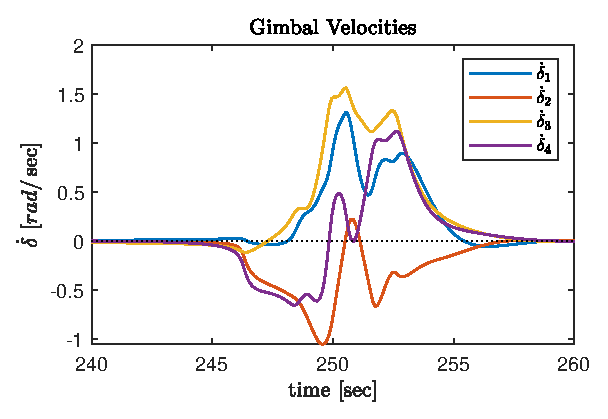
\includegraphics[width=1\columnwidth]{figures/plots/CMG/cm_reg_w10_zoom_delta_dot.eps}
    \caption{Gimbal velocities}
    \label{plt:cm_reg_w10_zoom_delta_dot}
\end{subfigure}
  %
  \begin{subfigure}[b]{0.49\columnwidth}
     \centering
    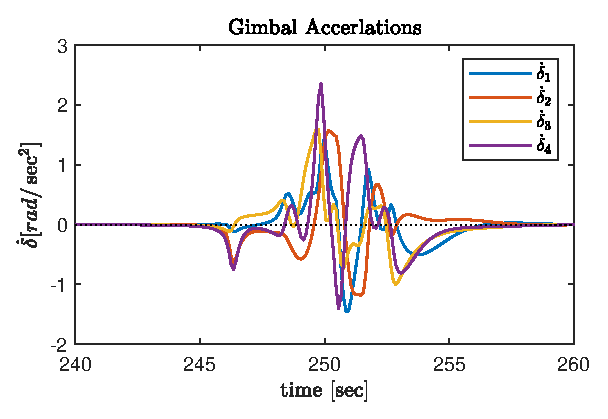
\includegraphics[width=1\columnwidth]{figures/plots/CMG/cm_reg_w10_zoom_delta_dot_dot.eps}
    \caption{Gimbal accerlations}
    \label{plt:cm_reg_w10_zoom_delta_dot_dot}
\end{subfigure}
\caption{Zoomed view of station keeping maneuver with CMG only ACS}
\label{plt:zoom_plots_omega_sing}

\end{figure}

\section{VSCMG based ACS}
In this section simulation results \acrlong{acs} based of complete \acrlong{vscmg} arranged in as pyramid cluster is discussed. Two types of simulations are performed first comparison with only CMG based ACS and later trajectory tracking maneuver is presented.

\section{Body rate regulation with VSCMG}
Considering same scenario of CMG only ACS discussed in previous section. We have deliberately set the gimbal configuration satellite state and initial angular velocity as shown in \autoref{tbl_cmg_at_sing} so that CMG is in singular state. Now advancing with same situation occurred with VSCMG based ACS. Controller gains and steering parameters are set as

\begin{equation}
\mathbf{Kq} =\begin{pmatrix}
300 & 0 & 0\\
0 & 300 & 0\\
0 & 0 & 300
\end{pmatrix} ;\quad \mathbf{Kw} =\begin{pmatrix}
850 & 0 & 0\\
0 & 850 & 0\\
0 & 0 & 850
\end{pmatrix}
\end{equation}

\noindent Notice selected gains are much higher than CMG only ACS. Bearing in mind that with higher gains were not Horowitz due to singularities present in CMG and bringing settling closer to 60 seconds was not possible. 
\noindent And constants for off-diagonal singularity robust steering law are 

\begin{equation*}
\begin{aligned}
\lambda  & =0.01\exp( -10m_{c})\\
\beta _{i} & =\min\left\{1\times 10^{3}\exp( -0.01m_{c} /m_{v}) ,\ 1000\right\}\\
\kappa  & =0.001\exp( -10m_{v})
\end{aligned}
\end{equation*}
 here $\beta_i $ is clipped to 1000  in order to avoid computational singularity when $m_v$ approaches zero. \begin{figure}[H]
     \centering
    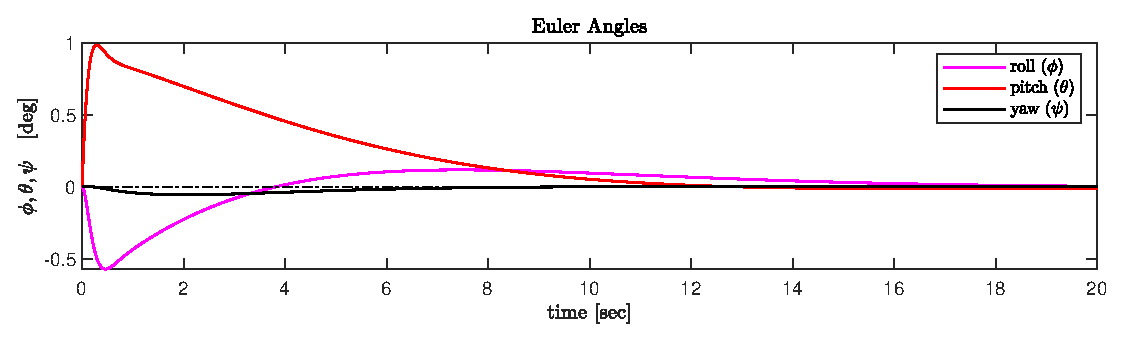
\includegraphics[width=0.9\columnwidth]{figures/plots/VSCMG/vs_reg_w10_ypr.eps}
    \caption{Euler angles for station keeping with VSCMG in vicinity of singularity}
    \label{plt:vs_reg_w10_ypr}
\end{figure}

\begin{figure}[H]
     \centering
    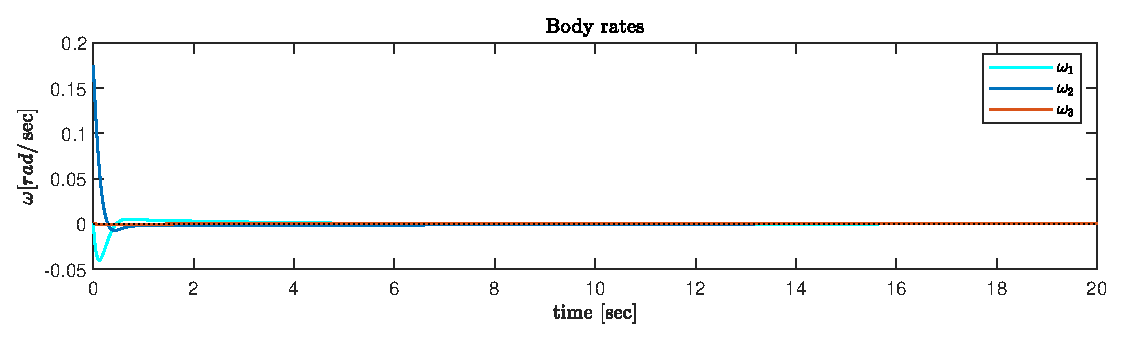
\includegraphics[width=0.9\columnwidth]{figures/plots/VSCMG/vs_reg_w10_w.eps}
    \caption{Body rates for station keeping with VSCMG in vicinity of singularity}
    \label{plt:vs_reg_w10_w}
\end{figure}
\noindent Upon initial disturbance Euler angles first rapidly increase but does not change more than $1 \degree$ due to high value of $ \textbf{K}_w $ and smoothly settles to desired state within 20 seconds as shown in \autoref{plt:vs_reg_w10_ypr}. Cancellation of velocity error verified from body rates shown in \autoref{plt:vs_reg_w10_w}

\begin{figure}[H]
     \centering
    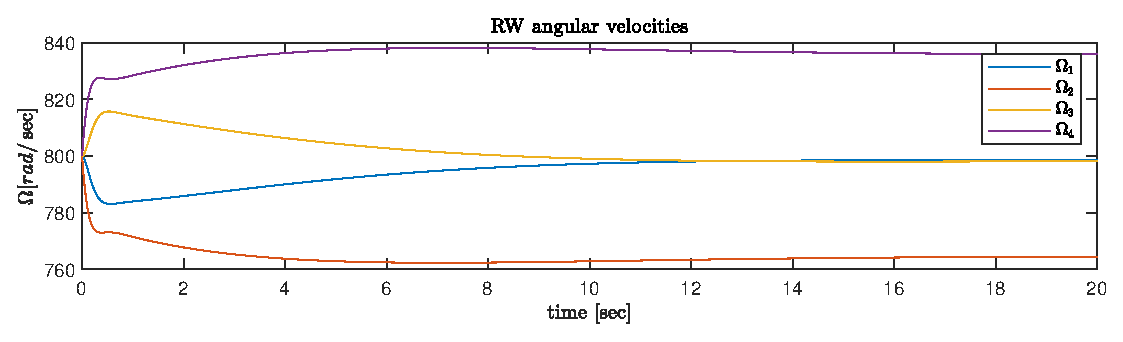
\includegraphics[width=0.9\columnwidth]{figures/plots/VSCMG/vs_reg_w10_Om.eps}
    \caption{RW rates for station keeping with VSCMG in vicinity of singularity}
    \label{plt:vs_reg_w10_Om}
\end{figure}

\begin{figure}[H]
     \centering
    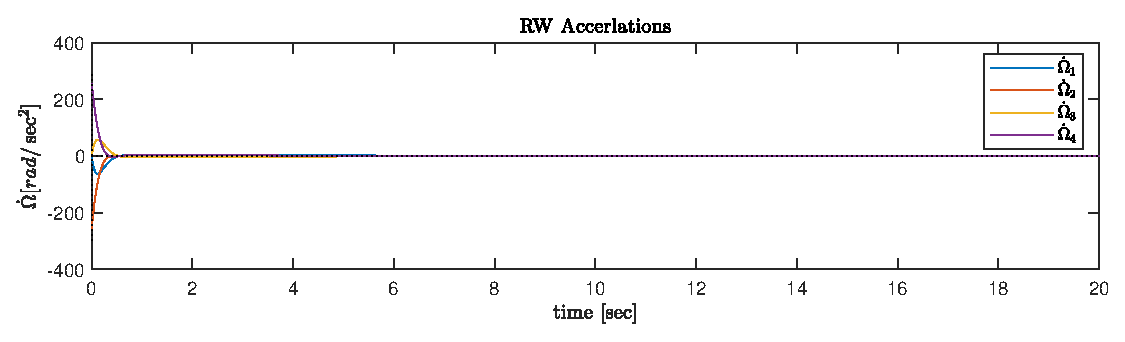
\includegraphics[width=0.9\columnwidth]{figures/plots/VSCMG/vs_reg_w10_Om_dot.eps}
    \caption{RW accelerations for station keeping with VSCMG in vicinity of singularity}
    \label{plt:vs_reg_w10_Om_dot}
\end{figure}
\noindent Despite RW change in velocities in \autoref{plt:vs_reg_w10_Om} are not too large, they are subjected to high accelerations shown in \autoref{plt:vs_reg_w10_Om_dot} with maximum magnitude if  $220\ rad/\sec^2$ which can be minimized with relaxed settling time criterion. At the same time gimbal velocities are considerably low which is evident due to high momentum of RW. Overall there is no chattering or high frequency components present in any of state despite existence of singularity.
\begin{figure}[H]
     \centering
    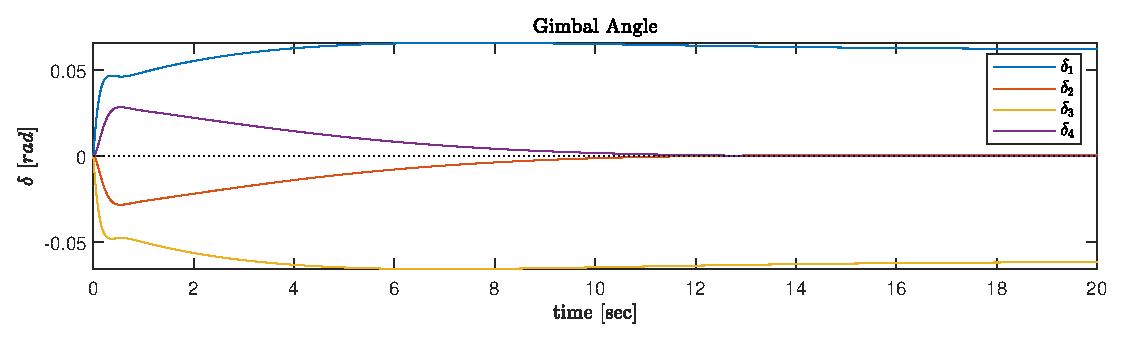
\includegraphics[width=0.9\columnwidth]{figures/plots/VSCMG/vs_reg_w10_delta.eps}
    \caption{Gimbal angles for station keeping with VSCMG in vicinity of singularity}
    \label{plt:vs_reg_w10_delta}
\end{figure}

\begin{figure}[H]
     \centering
    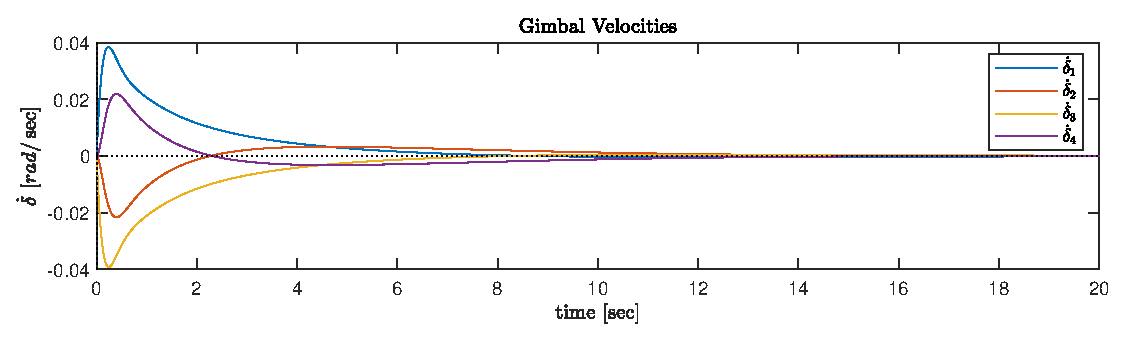
\includegraphics[width=0.9\columnwidth]{figures/plots/VSCMG/vs_reg_w10_delta_dot.eps}
    \caption{Gimbal velocities for station keeping with VSCMG in vicinity of singularity}
    \label{plt:vs_reg_w10_delta_dot}
\end{figure}

\section{Trajectory tracking with VSCMG ACS}
For verification of VSCMG based ACS and in order to test capabilities of steering law for large maneuvers for long period. An hypothetical scenario is assumed as a nadir pointing satellite in highly elliptical orbit has to maintain its payload towards earth. Since for elliptical satellite has to rotate at non constant speed in order to maintain its attitude with respect to true anomaly.
\newacronym{heo}{HEO}{Highly Elliptical Orbit}
Orbital parameters of ``MOLNIYA 1-86'' launched on 26 May 1993 by USSR is taken as reference satellite. A \acrlong{heo} with parameters shown in \autoref{tbl:MOLNIYA_param} was communications satellite used to test  a system of radio communications and television broadcasting using earth satellites as active transponders and to experiment with the system in practical use.\cite{Molniya}
\begin{table}[!h]
\centering
\begin{tabular}{p{0.30\textwidth}|p{0.20\textwidth}|p{0.15\textwidth}}
\toprule
 Parameter & Value & Unit \\
\midrule
 Inclination & 63.103 & $\displaystyle \deg$ \\
\hline 
 Eccentricity & 0.48485 & - \\
\hline 
 Semi major axis & 13353.0 & km \\
\hline 
 Apogee & 13457.1 & km \\
\hline 
 Perigee & 508.0 & km \\
\hline 
 Time period & 15354.2 & sec \\
 \bottomrule
\end{tabular}
\caption{MOLNIYA 1-86 Orbital details}
\label{tbl:MOLNIYA_param}
\end{table}

Reference trajectory in terms of Euler axis angle is realized by numerically solving Kepler equations of mean motion ($n$), Mean ($M$) Eccentric ($E$) and True anomaly
\begin{equation}
n=\sqrt{\frac{\mu }{a^{3}}}
\end{equation}
\begin{equation}
\begin{aligned}
M & =M_{0} +n( t-t_{0})\\
M & =E-e\sin E
\end{aligned}
\end{equation}
\begin{equation}
\tan\frac{\nu }{2} =\sqrt{\frac{1+e}{1-e}}\tan\frac{E}{2}
\end{equation}
Iterative solution is used to find mean anomalies for 10 periods of satellite to form a reference trajectory such that axis orthogonal to orbital plane is rotated by angle $\nu$ and quaternions are competed as

\begin{equation*}
q( t) =\left[\cos\frac{\nu ( t)}{2} ,0,0,\sin\frac{\nu ( t)}{2}\right]^{T}
\end{equation*}
Reference quaternions for Nine complete orbits are shown in \autoref{plt:molnia_ref_tack} and results of trajectory tracking are shown from \autoref{plt:vs_ref_mol_Om} to \autoref{plt:vs_ref_mol_Om}.

\begin{figure}[H]
     \centering
    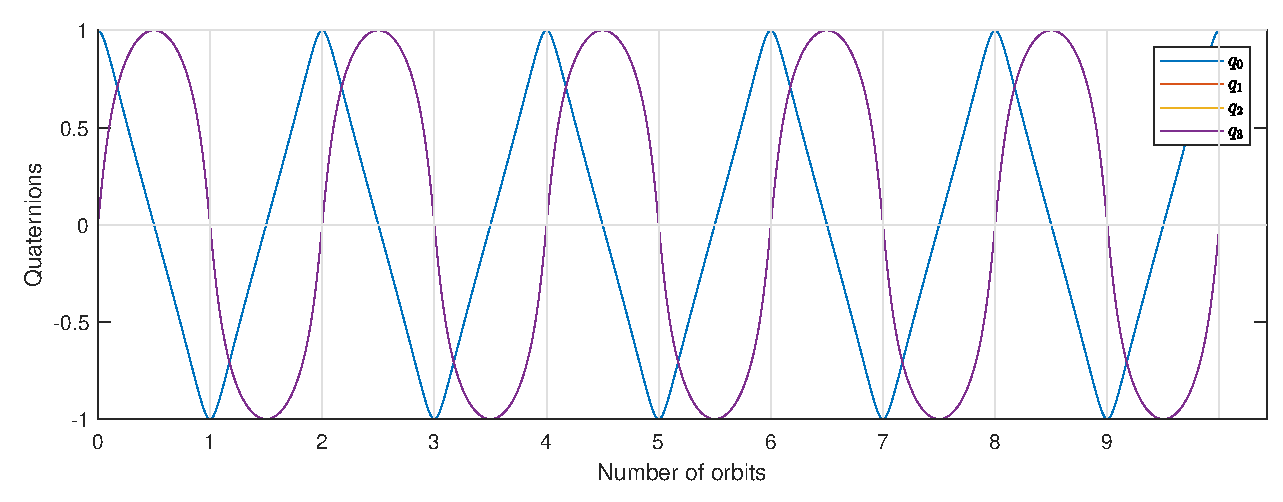
\includegraphics[width=0.9\columnwidth]{figures/plots/VSCMG/molnia_ref_tack.eps}
    \caption{Reference trajectory quaternions computed for MOLNIYA 1-86}
    \label{plt:molnia_ref_tack}
\end{figure}
\noindent Since trajectory tracked by satellite overlaps reference trajectory, least square residuals between reference quaternions and simulated quaternions are shown in \autoref{plt:vs_ref_mol_q_e} notice the deviation is within order of magnitude $10^{-6}$ 
\begin{figure}[H]
     \centering
    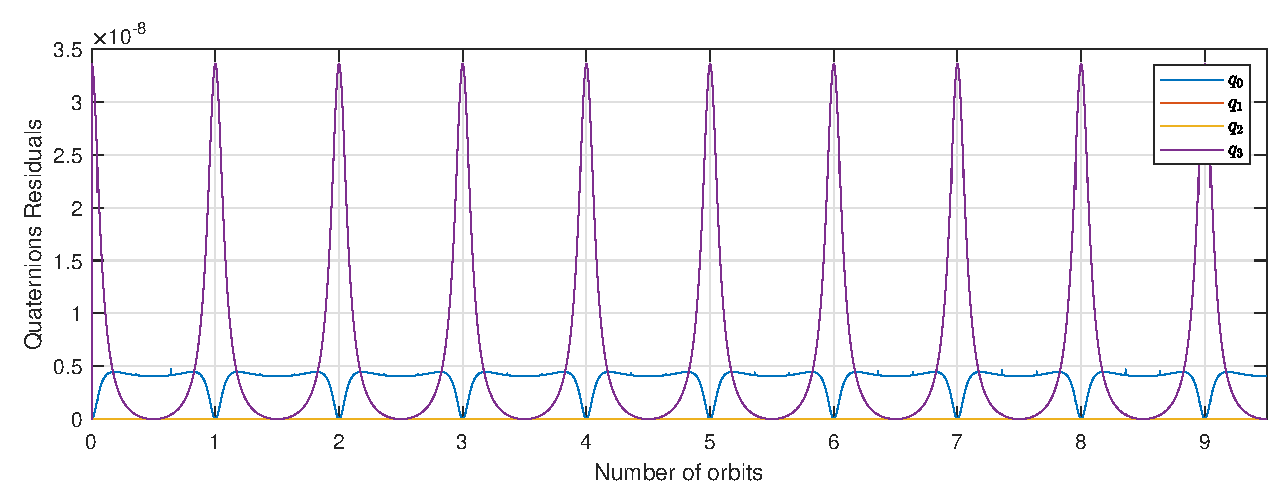
\includegraphics[width=0.9\columnwidth]{figures/plots/VSCMG/vs_ref_mol_q_e.eps}
    \caption{Least square residuals of quaternions computed for MOLNIYA 1-86}
    \label{plt:vs_ref_mol_q_e}
\end{figure}
\noindent Pitch and roll axis were placed in orbital plane, 9 complete revolutions are seen about yaw axis shown in \autoref{plt:vs_ref_mol_ypr}.
\begin{figure}[H]
     \centering
    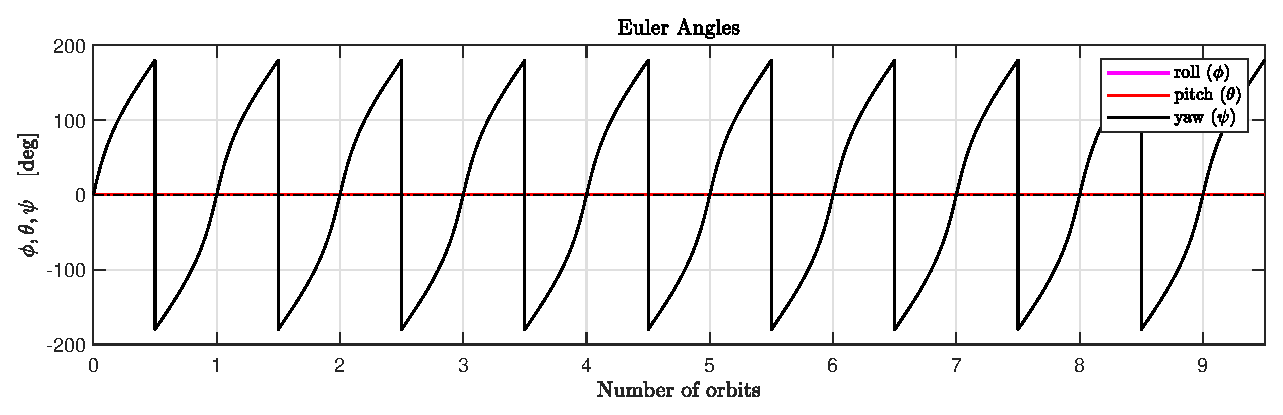
\includegraphics[width=0.9\columnwidth]{figures/plots/VSCMG/vs_ref_mol_ypr.eps}
    \caption{Euler angles computed for MOLNIYA 1-86}
    \label{plt:vs_ref_mol_ypr}
\end{figure}
Satellite orbital period is large and has to perform only one revolution per orbit due as a result body rates of tracked trajectory are very low. Although we can see from peaks at each orbit that rates slows down till apogee and accelerate till perigee.
\begin{figure}[H]
     \centering
    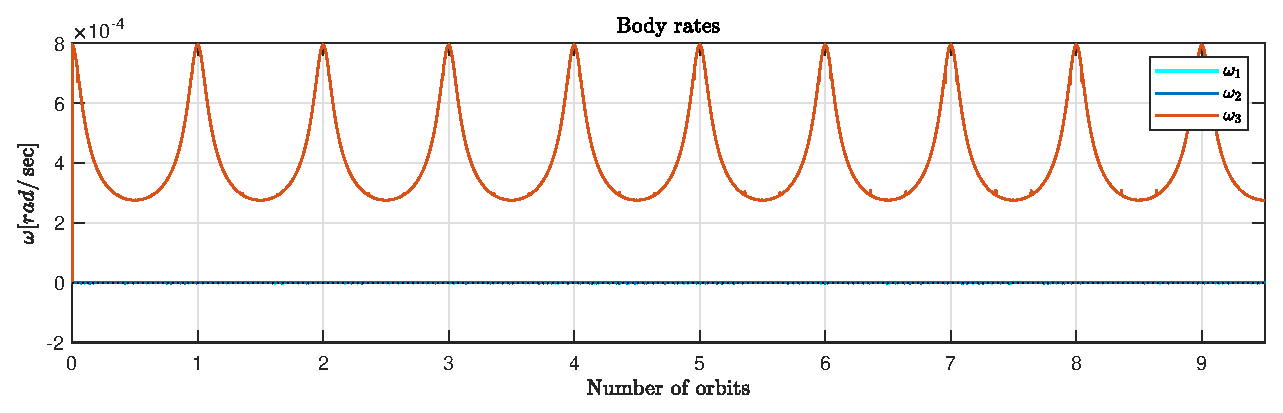
\includegraphics[width=0.9\columnwidth]{figures/plots/VSCMG/vs_ref_mol_w.eps}
    \caption{Body rates for trajectory tracking maneuver}
    \label{plt:vs_ref_mol_w}
\end{figure}
\noindent Similarly, in order to maintain varying body rate, RW velocities oscillate within magnitude of 0.2 $rad/sec$
\begin{figure}[H]
     \centering
    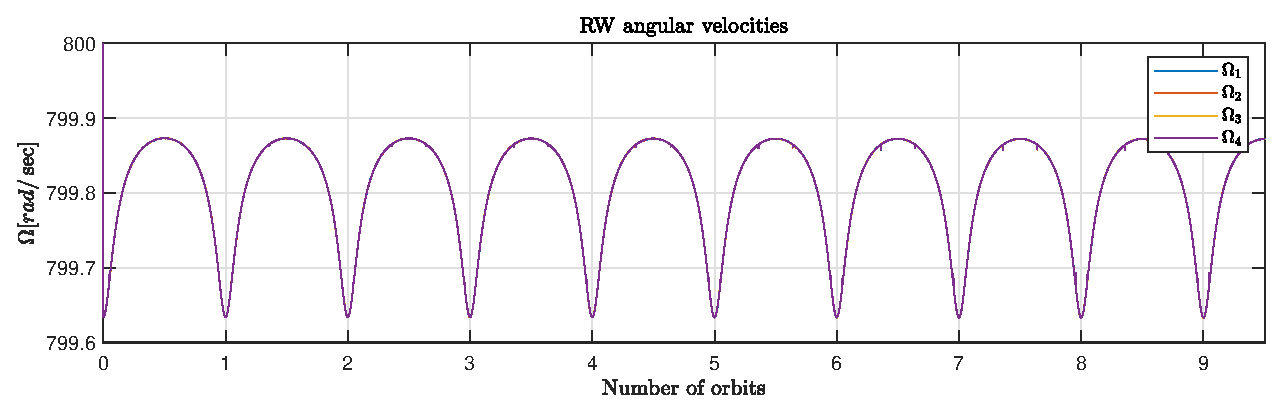
\includegraphics[width=0.9\columnwidth]{figures/plots/VSCMG/vs_ref_mol_Om.eps}
    \caption{RW angular velocity for trajectory tracking maneuver}
    \label{plt:vs_ref_mol_Om}
\end{figure}

From the results, it is clear that VSCMG based ACS are more beneficial than RW based and CMG based ACS. Clear advantages of VSCMG are listed below.

\begin{enumerate}
    \item VSCMG does not poses problem of singularities.
    \item they can produce large torque amplification like CMG,
    \item are able to steer away from singular state by using RWs.
    \item Moreover, Operation is smooth and gimbal rates are within permissible range and no impulsive motion or chattering occurs thus does not poses threat to mechanical integrity of system.
\end{enumerate}